% !TeX root = RJwrapper.tex
\title{ggplot2 Compatible Quantile-Quantile Plots in R}
\author{by Alexandre Almeida, Adam Loy, Heike Hofmann}

\maketitle

\abstract{%
Univariate distributional assessment is a common thread throughout
statistical analyses during both the exploratory and confirmatory
stages. Q-Q plots compare two distributions by matching a common set of
quantiles and displaying them as a scatterplot. To aid in the
interpretation of Q-Q plots, reference lines and confidence bands are
often added. Another approach to aid in interpretation is to detrend the
Q-Q plot so the vertical comparisons of interest are the focus. While
various implementations of Q-Q plots exist in R, none implement all of
these features. \pkg{qqplotr} extends \pkg{ggplot2} to provide a
complete implementation of Q-Q plots. This paper introduces the plotting
framework provided by \pkg{qqplotr} and provides multiple examples of
how it can be used.
}

\newcommand{\hh}[1]{{\textcolor{orange}{#1}}}
\newcommand{\al}[1]{{\textcolor{violet}{#1}}}
\newcommand{\Aa}[1]{{\textcolor{olive}{#1}}}

\subsection{TODO:}\label{todo}

\begin{itemize}
\tightlist
\item
  Be consistent with:

  \begin{itemize}
  \tightlist
  \item
    Indentation rules for code.
  \item
    Colors/themes/sizes for the plots.
  \item
    Use ``normal'' when not specifying (as in ``a normal
    distribution''). Use ``Normal'' when specifying (as in ``the
    Standard Normal Distribution'').
  \item
    Use ``colour'' instead of ``color'' when using ggplot2 functions due
    to compatibility reasons.
  \item
    Dashing punctuation: use em dashes (---) instead of en dashes (--).
    Don't place spaces before or after them.
  \end{itemize}
\end{itemize}

\subsection{Background}\label{background}

\label{sec:background}

Univariate distributional assessment is a common thread throughout
statistical analyses during both the exploratory and confirmatory
stages. When we begin exploring a new data set we often consider the
distribution of individual variables before moving on to explore
multivariate relationships. After a model has been fit to a data set, we
must assess whether the distributional assumptions made are reasonable,
and if they are not, then we must understand the impact this has on the
conclusions of the model. Graphics provide arguably the most common way
to carry out these univariate assessments. While there are many plots
that can be used for distributional exploration and assessment, a
quantile-quantile (Q-Q) plot \citep{Wilk1968-ii} is one of the most
common plots used.

Q-Q plots compare two distributions by matching a common set of
quantiles. To compare a sample, \(y_1, y_2, \ldots, y_n\), to a
theoretical distribution, a Q-Q plot is simply a scatterplot of the
sample quantiles, \(y_{(i)}\), against the corresponding quantiles from
the theoretical distribution, \(F^{-1}\left( F_n(y_{(i)}) \right)\). If
the empirical distribution is consistent with the theoretical
distribution, then the Q-Q plot will be linear. For example,
Figure\textasciitilde{}\ref{fig:ex-qq1} shows two Q-Q plots: the left
plot compares a sample drawn from a lognormal distribution to a
lognormal distribution, while the right plot compares a sample drawn
from a lognormal distribution to a normal distribution. As expected, the
lognormal Q-Q plot is approximately linear, as the data and model are in
agreement, while the normal Q-Q plot is curved, indicating disagreement
between the data and the model.

\begin{Schunk}
\begin{figure}

{\centering 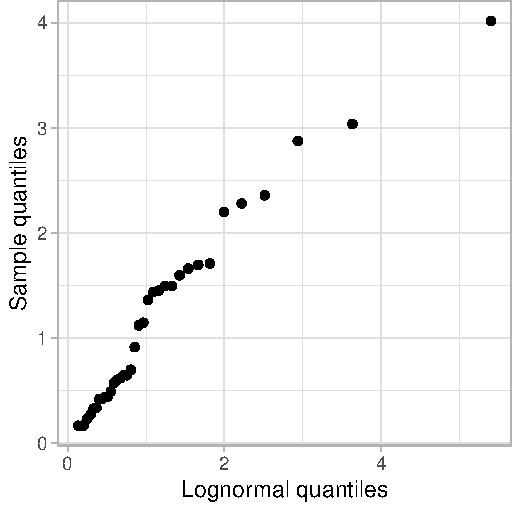
\includegraphics[width=.4\linewidth]{qqplotr_files/figure-latex/ex-qq1-1} 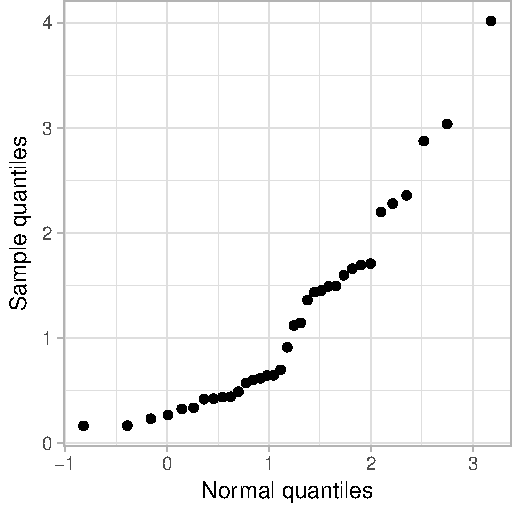
\includegraphics[width=.4\linewidth]{qqplotr_files/figure-latex/ex-qq1-2} 

}

\caption[The left plot compares a sample drawn from a lognormal distribution to a lognormal distribution, while the right plot compares a sample drawn from a lognormal distribution to a normal distribution]{The left plot compares a sample drawn from a lognormal distribution to a lognormal distribution, while the right plot compares a sample drawn from a lognormal distribution to a normal distribution. The curvature in the normal Q-Q plot highlights the disagreement betweeen the data and the model.}\label{fig:ex-qq1}
\end{figure}
\end{Schunk}

Additional graphical elements are often added to Q-Q plots in order to
aid in distributional assessment. A reference line is often added to a
Q-Q plot to help detection of departures from the proposed model. This
line is often drawn either by tracing the identity line or by connecting
two pairs of quantiles, such as the first and third quartiles. Pointwise
or simultaneous confidence bands are also frequently built around the
reference line to display the expected degree of sampling error for the
proposed model. Such bands help gauge how troubling a departure from the
proposed model may be. Figure\textasciitilde{}\ref{fig:ex-qq2} adds
identity reference lines and 95\% pointwise confidence bands to the Q-Q
plots in Figure\textasciitilde{}\ref{fig:ex-qq1}.

\begin{Schunk}
\begin{figure}

{\centering 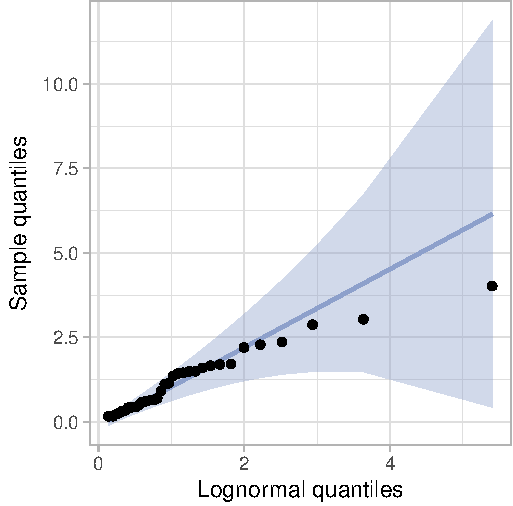
\includegraphics[width=.4\linewidth]{qqplotr_files/figure-latex/ex-qq2-1} 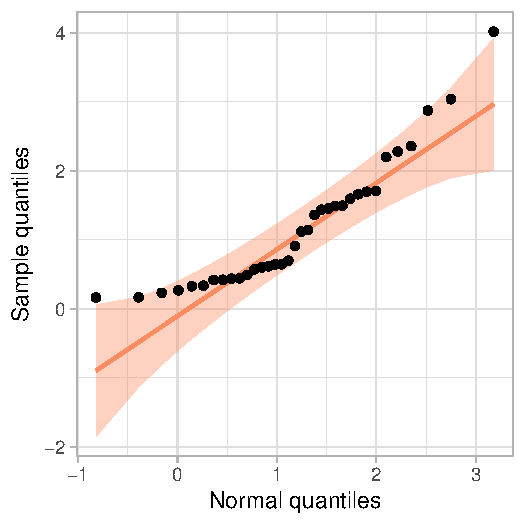
\includegraphics[width=.4\linewidth]{qqplotr_files/figure-latex/ex-qq2-2} 

}

\caption[Adding reference lines and $95\%$ pointwise confidence bands to the Q-Q plots in Figure 1]{Adding reference lines and $95\%$ pointwise confidence bands to the Q-Q plots in Figure 1.}\label{fig:ex-qq2}
\end{figure}
\end{Schunk}

Different orientations of Q-Q plots have also been proposed, most
notably the detrended Q-Q plot. To detrend a Q-Q plot, the \(y\)-axis is
changed to show the difference between the observed quantile and the
reference line. Consequently, the line representing agreement with the
theoretical distribution is the \(x\)-axis. \citet{Loy2016-fg} find that
detrended Q-Q plots are more powerful than other designs, as long as the
\(x\)- and \(y\)-axes are adjusted to ensure that distances in the
\(x\)- and \(y\)-directions are on the same scale. This Q-Q plot design
is called an \emph{adjusted detrended Q-Q plot}. Without this adjustment
to the range of the axes \emph{ordinary detrended Q-Q plots} are
produced, which were found to have lower power than the standard Q-Q
plot in some situations \citep{Loy2016-fg}, while the adjusted detrended
Q-Q plots were found to be more powerful.
Figure\textasciitilde{}\ref{fig:ex-detrend} displays the Q-Q plot from
Figure\textasciitilde{}\ref{fig:ex-qq2} along with its adjusted
detrended version.

\begin{Schunk}
\begin{figure}

{\centering 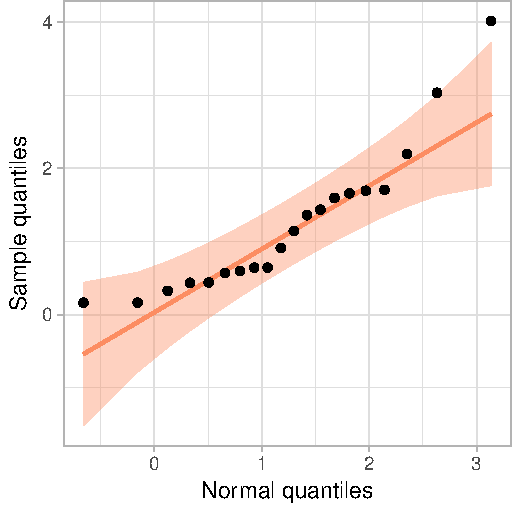
\includegraphics[width=.4\linewidth]{qqplotr_files/figure-latex/ex-detrend-1} 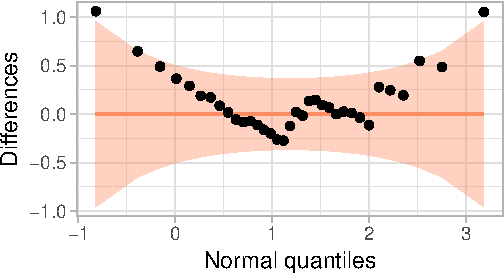
\includegraphics[width=.4\linewidth]{qqplotr_files/figure-latex/ex-detrend-2} 

}

\caption[The left plot displays a traditional normal Q-Q plot for data simulated from a lognormal distribution]{The left plot displays a traditional normal Q-Q plot for data simulated from a lognormal distribution. The right plot displays an adjusted detrended Q-Q plot of the same data, created by plotting the differences between the sample quantiles and the proposed model on the $y$-axis.}\label{fig:ex-detrend}
\end{figure}
\end{Schunk}

Various implementations of Q-Q plots exist in R. Normal Q-Q plots, where
a sample is compared to the Standard Normal Distribution, are
implemented using \texttt{qqplot} and \texttt{qqline} in \pkg{base}
graphics \citep{R}. \pkg{lattice} provides a general framework for Q-Q
plots in the \texttt{qqmath} function, allowing one to compare a sample
to any theoretical distribution by specifying the appropriate quantile
function \citep{lattice}. \texttt{qqPlot} in the \pkg{car} package also
allows for the assessment of non-normal distributions and adds pointwise
confidence bands via normal theory or the parametric bootstrap
\citep{car}. \pkg{ggplot2} provides \texttt{geom\_qq} and
\texttt{geom\_qq\_line}, enabling the creation of Q-Q plots with a
reference line, much like those created using \texttt{qqmath}
\citep{ggplot2}. None of these general-use packages allow for easy
construction of detrended Q-Q plots.

\pkg{qqplotr} extends \pkg{ggplot2} to provide a complete implementation
of Q-Q plots. The package allows for quick construction of all Q-Q plot
designs without sacrificing the flexibility of the \pkg{ggplot2}
framework. In the remainder of this paper, we introduce the plotting
framework provided by \pkg{qqplotr} and provide multiple examples of how
it can be used.

\subsection{\texorpdfstring{Implementing Q-Q plots in the \pkg{ggplot2}
framework}{Implementing Q-Q plots in the  framework}}\label{implementing-q-q-plots-in-the-framework}

\label{sec:implementing}

\pkg{qqplotr} provides a \pkg{ggplot2} layering mechanism for Q-Q
points, lines, and confidence bands by implementing separate statistical
transformations (\texttt{stat}s). In this section, we describe each
transformation.

\subsubsection{\texorpdfstring{\texttt{stat\_qq\_point}}{stat\_qq\_point}}\label{stat_qq_point}

This modified version of \texttt{stat\_qq}/\texttt{geom\_qq} (from
\pkg{ggplot2}) plots the sample quantiles versus the theoretical
quantiles (as done in Figure\textasciitilde{}\ref{fig:ex-qq1}). The
novelty of this implementation is an option to detrend the plotted
points. Note that all other transformations in the \pkg{qqplotr} package
also allow for the detrend option. Below we present a complete call to
\texttt{stat\_qq\_point} and highlight the default values of its
parameters:

\begin{Schunk}
\begin{Sinput}
stat_qq_point(
  data = NULL,
  mapping = NULL,
  geom = "point",
  position = "identity",
  na.rm = TRUE,
  show.legend = NA,
  inherit.aes = TRUE,
  distribution = "norm",
  dparams = list(),
  detrend = FALSE,
  identity = TRUE,
  qtype = 7,
  qprobs = c(0.25, 0.75),
  ...
  )
\end{Sinput}
\end{Schunk}

\begin{itemize}
\item
  Parameters such as \texttt{data}, \texttt{mapping}, \texttt{geom},
  \texttt{position}, \texttt{na.rm}, \texttt{show.legend}, and
  \texttt{inherit.aes} are commonly found among several \pkg{ggplot2}
  transformations.
\item
  \texttt{distribution} is a character string that sets the theoretical
  probability distribution. Here, we followed the nomenclature from the
  \pkg{stats} package, but rather than requiring the full function name
  for a distribution (e.g., \texttt{"dnorm"}), only the suffix is
  required (e.g., \texttt{"norm"}). If you wish to provide a custom
  distribution, then you must first create its density (PDF),
  distribution (CDF), quantile, and simulation functions, following the
  nomenclature outlined in the \pkg{stats} package. For example, for
  \texttt{"custom"}, you must provide the \texttt{dcustom},
  \texttt{pcustom}, \texttt{qcustom}, and \texttt{rcustom} functions. A
  detailed example is given in the \nameref{sec:user-dists} section.
\item
  \texttt{dparams} is a named list specifying the parameters of the
  proposed \texttt{distribution}. By default, maximum likelihood
  etimates (MLEs) are used, so this argument overrides this default.
  Please note that MLEs are currently only supported for distributions
  available in the \pkg{stats} package, so if a custom distribution is
  provided to \texttt{distribution}, then \emph{all} of its parameters
  have to be estimated somehow and passed as a named list to
  \texttt{dparams}.
\item
  \texttt{detrend} is a logical that controls whether the points should
  be detrended (as shown in
  Figure\textasciitilde{}\ref{fig:ex-detrend}). For additional details,
  see the \nameref{sec:detrending} section.
\item
  \texttt{identity} is only used when \texttt{detrend\ =\ TRUE}. This
  parameter is a logical that controls if the identity line should be
  used as the reference line when constructing the detrended Q-Q plot.
  By default, the identity reference line is used. If
  \texttt{identity\ =\ FALSE}, then the points will be detrended
  according to the traditional Q-Q line that intersects the two data
  quantiles specified in \code{qprobs}
\item
  \texttt{qtype} and \texttt{qprobs} are only used when
  \texttt{detrend\ =\ TRUE} and \texttt{identity\ =\ FALSE}. These
  parameters are passed onto the \texttt{type} and \texttt{probs}
  parameters of the \texttt{quantile} function from \pkg{stats}, both of
  which are used to specify which quantiles that the reference line
  (i.e., the proposed model) passes through.
\end{itemize}

\subsubsection{\texorpdfstring{\texttt{stat\_qq\_line}}{stat\_qq\_line}}\label{stat_qq_line}

\Aa{This statistical transformation draws a reference line based on the identity line or two sample quantiles.}

\begin{Schunk}
\begin{Sinput}
stat_qq_line(
  data = NULL,
  mapping = NULL,
  geom = "path",
  position = "identity",
  na.rm = TRUE,
  show.legend = NA,
  inherit.aes = TRUE,
  distribution = "norm",
  dparams = list(),
  detrend = FALSE,
  identity = TRUE,
  qtype = 7,
  qprobs = c(0.25, 0.75),
  ...
  )
\end{Sinput}
\end{Schunk}

Nearly all of the parameters for \texttt{stat\_qq\_line} are identical
to those for \texttt{stat\_qq\_point}. The one exception is
\texttt{identity}, which has a slightly different interpretation. In
\texttt{stat\_qq\_line}, \texttt{identity} is \emph{always} used,
regardless of the value of \texttt{detrend}. This parameter controls
which reference line is drawn:

\begin{enumerate}
\def\labelenumi{\alph{enumi})}
\tightlist
\item
  When \texttt{identity\ =\ TRUE}, the \emph{identity line} is drawn. By
  definition of a Q-Q plot the \emph{identity line} represents the
  theoretical distribution.
\item
  When \texttt{identity\ =\ FALSE}, the \emph{Q-Q line} is drawn. This
  line estimates the empirical distribution.
\end{enumerate}

The intercept and slope of these lines relate to the mean and scale
parameters of the theoretical and the empirical distributions,
respectively. By comparing these two lines we learn about how well the
parameters estimated from the sample match the theoretical parameters.
For a distributional family that is invariant to linear transformations,
the parameters specified in the theoretical distribution only have an
effect on the Q-Q line and the Q-Q points---that is, the parameters get
shifted and scaled in the plot, but relative relationships do not change
aside from a change in scales. For other distributions, such as a
lognormal distribution, re-specifications of the parameters result in
non-linear transformations of the Q-Q line and Q-Q points (see
Figure\textasciitilde{}\ref{fig:qqline} for an example).

\begin{Schunk}
\begin{figure}
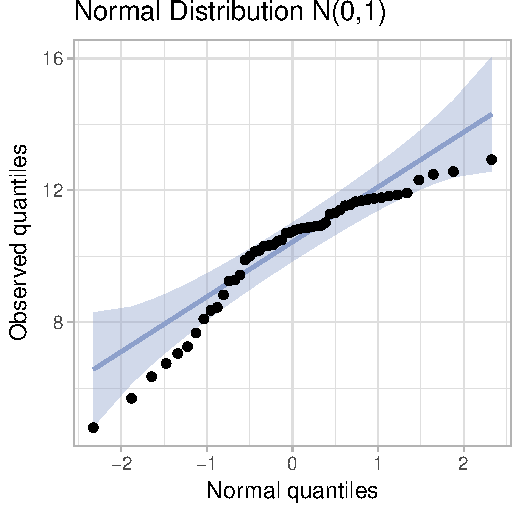
\includegraphics[width=\textwidth]{qqplotr_files/figure-latex/qqline-1} \caption{Q-Q plots of (top-left) a mis-specified normal distribution, (top-right) a normal distribution with ML parameter estimates. Between these two plots only the scales on the axes change. The bottom two plots show Q-Q plots of the same sample from a lognormal distribution. On the left, the theoretical distribution is mis-specified with a mean of 0 and variance of 1. On the right, ML estimates for mean and variance are used. \Aa{AA: The two left hand side plots are different from before as an effect of the new identity referece line. Even though this was not what we originally wanted to show with this figure, I find that these new plots show exactly why using the identity line vs. the traditional Q-Q line is important in our package, which uses MLEs by default. It can serve as a good illustration.}}\label{fig:qqline}
\end{figure}
\end{Schunk}

\Aa{AA: I suppose we need to rework the following paragraph, since the identity line is now used as default:}

\al{I found myself asking if the paragraph below was necessary/out of place now that we have made some changes to the package and adjusted the above exposition.}

By default the Q-Q line is drawn through two points, corresponding to
the .25 and .75 quantiles of the distributions on \(x\) (theoretical
distribution) and \(y\) (empirical distribution). While we are using
MLEs to identify the theoretical distribution, these estimates are only
used in determining the \(x\)-coordinates of these points. For the \(y\)
coordinates, the 1st and 3rd quartiles are used by default for more
robust estimation. Therefore, the difference between the observed and
theoretical distributions presents itself in the difference between the
Q-Q line and the identity line. Using robust estimates for the Q-Q line
is of particular advantage for small samples \citep{Loy2016-fg}.

\subsubsection{\texorpdfstring{\texttt{stat\_qq\_band}}{stat\_qq\_band}}\label{stat_qq_band}

Confidence bands can be drawn around the reference line using one of
three methods: a normal approximation, the parametric bootstrap, or the
tail-sensitive procedure \citep{Aldor-Noiman2013-xw}. Below, we present
the call to \texttt{stat\_qq\_band} and describe its specific
parameters:

\begin{Schunk}
\begin{Sinput}
stat_qq_band(
  data = NULL,
  mapping = NULL,
  geom = "qq_band",
  position = "identity",
  show.legend = NA,
  inherit.aes = TRUE,
  na.rm = TRUE,
  distribution = "norm",
  dparams = list(),
  detrend = FALSE,
  identity = TRUE,
  qtype = 7,
  qprobs = c(0.25, 0.75),
  bandType = "normal",
  B = 1000,
  conf = 0.95,
  mu = NULL,
  sigma = NULL,
  ...
  )
\end{Sinput}
\end{Schunk}

\begin{itemize}
\item
  \texttt{bandType} is a character string controlling the method used to
  construct the confidence bands:

  \begin{itemize}
  \tightlist
  \item
    \textbf{Normal:} Specifying \texttt{bandType\ =\ "normal"}
    constructs pointwise confidence bands based on a normal
    approximation to the distribution of the order statistics. For
    example, an approximate 95\% confidence interval for the \(i\)th
    order statistic is
    \linebreak \(\widehat{X}_{(i)}~\pm~\Phi^{-1}(.975)~\cdot~SE(X_{(i)})\),
    where \(\widehat{X}_{(i)}\) denotes the value along the fitted
    reference line, \(\Phi^{-1}(\cdot)\) denotes the quantile function
    for the Standard Normal Distribution, and \(SE(X_{(i)})\) is the
    standard error of the \(i\)th order statistic.
  \item
    \textbf{Bootstrap:} Specifying \texttt{bandType\ =\ "boot"}
    constructs pointwise confidence bands using percentile confidence
    intervals from the parametric bootstrap.
  \item
    \textbf{Tail-sensitive:} Specifying \texttt{bandType\ =\ "ts"}
    constructs the simulation-based tail-sensitive simultaneous
    confidence bands proposed by \citet{Aldor-Noiman2013-xw}.
    \al{Currently, TS bands are only implemented for `distribution = norm`.}
  \end{itemize}
\item
  \texttt{B} is a dual-purpose integer parameter: it specifies the
  number of bootstrap replicates, if \texttt{bandType\ =\ "boot"}, or
  the number of simulated samples if \texttt{bandType\ =\ "ts"}.
\item
  \texttt{conf} is a numerical variable, bound between 0 and 1, that
  sets the confidence level of the bands.
\item
  \texttt{mu} and \texttt{sigma} are only used when
  \texttt{bandType\ =\ "ts"}. They represent the center and scale
  parameters, respectively, used to construct the simulated
  tail-sensitive confidence bands. If either is \texttt{NULL}, then
  \emph{both} the center and scale parameters will be estimated using
  robust estimates via \pkg{robustbase} \citep{robustbase}.
\end{itemize}

\subsubsection{\texorpdfstring{Groups in
\texttt{qqplotr}}{Groups in qqplotr}}\label{groups-in-qqplotr}

\texttt{qqplotr} is implemented in accordance with the \texttt{ggplot2}
concept of groups. When the user maps values to aesthetics that
explicitly (by using \texttt{group}) or implicitly (such as
\texttt{shape} or discrete values of \texttt{colour}, \texttt{size}
etc.) introduce groups, the corresponding calculations respect the
grouping in the data. All groups are compared to the same distributional
family, but the parameters are estimated \emph{separately} for each of
the groups (given that \texttt{dparams\ =\ NULL}). If the user wants to
fit the \emph{same} distribution (i.e., same parameter estimates) to
each group, then the estimates must be manually calculated and passed to
\texttt{dparams} as a named list for each of the desired \pkg{qqplotr}
transformations. The use of groups is illustrated in more detail in the
\nameref{sec:brfss} section.

\FloatBarrier

\subsection{Examples}\label{examples}

\label{sec:examples}

In this section, we demonstrate the capabilities of the \pkg{qqplotr}
package by provide multiple examples of how the package can be used. We
start by loading the package:

\begin{Schunk}
\begin{Sinput}
library(qqplotr)
\end{Sinput}
\end{Schunk}

\subsubsection{\texorpdfstring{Constructing Q-Q plots with
\texttt{qqplotr}}{Constructing Q-Q plots with qqplotr}}\label{constructing-q-q-plots-with-qqplotr}

To give a brief introduction on how to use \pkg{qqplotr} and its
transformations, consider the \texttt{urine} dataset from \pkg{boot}.
This small dataset consists of 79 urine specimens that were analyzed to
determine if certain physical characteristics of the urine (e.g., pH or
urea concentration) might be related to the formation of calcium oxalate
crystals. In this example, we focus on the distributional assessment of
pH measurements made on the samples.

We start by plotting a normal Q-Q plot of the data. The top-left plot in
Figure\textasciitilde{}\ref{fig:urine-qq-bands} shows the Q-Q plot of
the pH measurements versus the normal distribution quantiles. As
previously described, the theoretical distributional parameters are
estimated on the fly with MLEs. By default, \texttt{stat\_qq\_band}
creates pointwise confidence bands based on the normal approximation
(\texttt{bandType\ =\ "normal"}) of the order statistics distribution.
As we can see, the urine pH measurements distribution for this dataset
is lightly right-skewed.

As previously discussed, three distinct approaches are availble in
\pkg{qqplotr} to construct the confidence bands. The top row from
Figure\textasciitilde{}\ref{fig:urine-qq-bands} presents three plots
with the different confidence bands drawn over the same normal Q-Q
points and identity lines. The bottom row from
Figure\textasciitilde{}\ref{fig:urine-qq-bands} presents the detrended
version of the those plots.

\al{The next paragraph is confusing. If we want to talk about a specific point, then we should highlight it on the plots using a different color. This will help reduce cognitive load on the reader. Also, the final conclusion from the TS version seems off: when using simultaneous bands, we would reject normality if a point is outside the bands, whereas we are unlikely to do so using pointwise bands (if you assume the analyst knows a bit about probability). We should clean up this discussion a bit.}

When assessing the tail-sensitive confidence bands (bottom-right), we
can see that an additional point is inside the confidence bands when
compared to the normal (bottom-left) and the bootstrap confidence bands
methods (bottom-center). In addition, the points from the distribution
center of mass are also more distant from tail-sensitive confidence
bands limits when compared to the other methods. Hence, one could
conclude by looking at the tail-sensitive plot at the bottom-right that,
even though the normal distribution seems like a slightly rough
approximation, the assumption of normality is reasonable for the urine
pH measurements. By inspecting the other confidence bands methods, in
turn, one might be in doubt about the assumption of normality.

\begin{Schunk}
\begin{figure}

{\centering 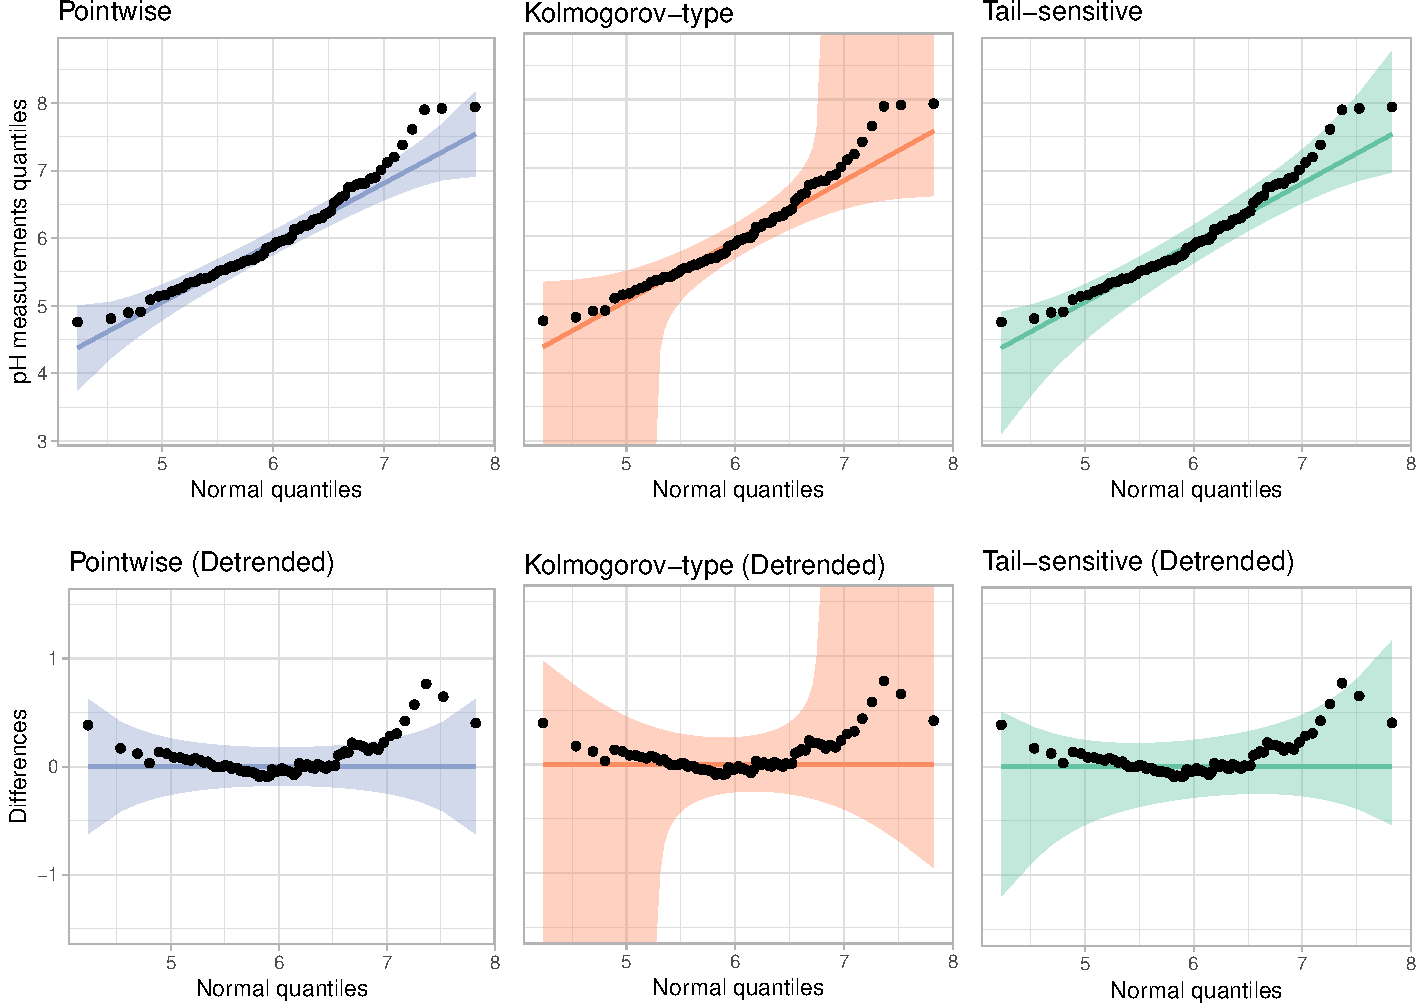
\includegraphics[width=1.0\textwidth]{qqplotr_files/figure-latex/urine-qq-bands-1} 

}

\caption{Normal Q-Q plots of pH measurements from urine samples using different confidence bands. Depending on the type of confidence band used, we come to different conclusions. \Aa{AA: Not sure about how much (and if) to include of the code chunk used to produce these plots.}}\label{fig:urine-qq-bands}
\end{figure}
\end{Schunk}

\FloatBarrier

\subsubsection{User-provided
distributions}\label{user-provided-distributions}

\label{sec:user-dists}

Using the capabilities of \pkg{qqplotr} with the distributions
implemented in the \pkg{stats} package is relatively straightfoward,
since the implementation allows you to specify the suffix (i.e.,
distribution and or abbreviation) via the \texttt{distribution} argument
and the parameter estimates via the \texttt{dparams} argument. However,
there are times when the distributions in \pkg{stats} are not sufficient
for the demands of the analysis. For example, there is no left-skewed
distribution listed
\al{aside from the Beta Distribution, which has a restrictive support.}
User-coded distributions, or distributions from other packages, can be
used with \pkg{qqplotr} as long as the distributions are defined
following the conventions laid out in the \pkg{stats} package.
Specfically, for some distribution there must be density/mass
(\texttt{d} prefix), CDF (\texttt{p} prefix), quantile (\texttt{q}
prefix), and simulation (\texttt{r} prefix) functions. In this section,
we illustrate the use of the smallest extreme value distribution (SEV).

To qualify for the 2012 Olympics in the men's long jump, athletes had to
meet/exceed the 8.1 meter standard or place in the top twelve. During
the qualification events, each athlete was able to jump up to three
times, using their best (i.e., longest) jump as the result.
Figure\textasciitilde{}\ref{fig:jump-density} shows a density plot of
the results, which are clearly left skewed.

\begin{Schunk}
\begin{figure}

{\centering 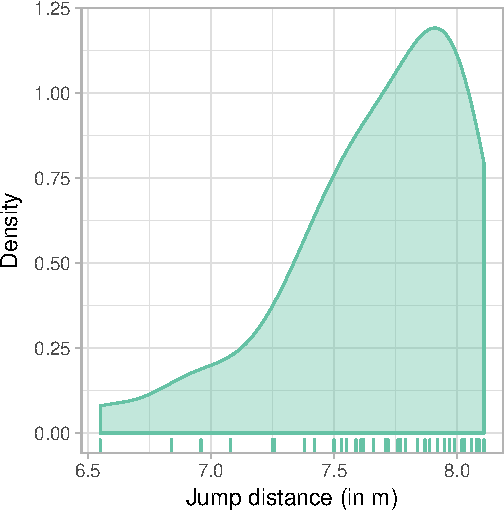
\includegraphics[width=0.45\textwidth]{qqplotr_files/figure-latex/jump-density-1} 

}

\caption[Density plot of the 2012 men's long jump qualifying round]{Density plot of the 2012 men's long jump qualifying round. The distances are clearly left skewed.}\label{fig:jump-density}
\end{figure}
\end{Schunk}

In order to model the jump distances we must first define a left-skewed
distribution. Below, we define the suite of distributional functions
necessary to utilize the SEV distribution.

\begin{Schunk}
\begin{Sinput}
# CDF
psev <- function(q, mu = 0, sigma = 1) {
    z <- (q - mu) / sigma
    1 - exp(-exp(z))
}

# PDF
dsev <- function(x, mu = 0, sigma = 1) {
  z <- (x - mu) / sigma
  (1 / sigma) * exp(z - exp(z))
}

# Quantile function
qsev <- function(p, mu = 0, sigma = 1) {
  mu + log(-log(1 - p)) * sigma
}

# Simulation function
rsev <- function(n, mu = 0, sigma = 1) {
  qsev(runif(n), mu, sigma)
}
\end{Sinput}
\end{Schunk}

With the \texttt{*sev} distribution functions in hand, we can create a
Q-Q plot to assess the appropriateness of the SEV model
(Figure\textasciitilde{}\ref{fig:sev-qq}). The Q-Q plot shows that the
distances do not substantially deviate from the SEV model, so we have
found an adequate representation of the distances. The code used to
create Figure\textasciitilde{}\ref{fig:sev-qq} is given below:

\begin{Schunk}
\begin{Sinput}
ggplot(longjump, aes(sample = distance)) +
  stat_qq_band(
    distribution = "sev", 
    identity = FALSE,
    dparams = list(mu = 0, sigma = 1), 
    alpha = 0.3
    ) +
  stat_qq_line(
    distribution = "sev", 
    identity = FALSE,
    dparams = list(mu = 0, sigma = 1)
    ) +
  stat_qq_point(
    distribution = "sev", 
    dparams = list(mu = 0, sigma = 1)
    ) +
  xlab("Theoretical quantiles") +
  ylab("Jump distance (in m)") +
  theme_bw()
\end{Sinput}
\begin{figure}

{\centering 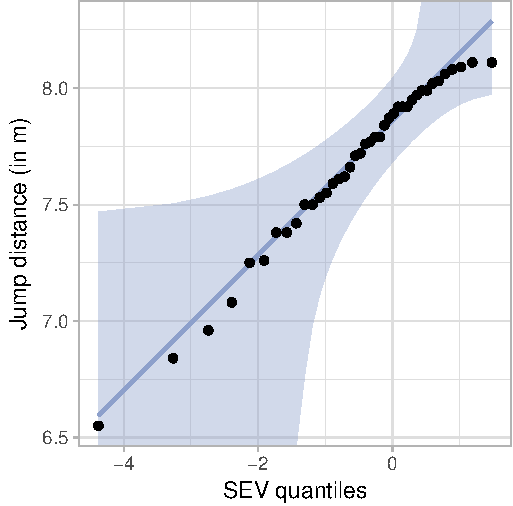
\includegraphics[width=0.45\textwidth]{qqplotr_files/figure-latex/sev-qq-1} 

}

\caption[Q-Q plot comparing the long jump distances to the standard SEV distribution with 95\% pointwise confidence bands]{Q-Q plot comparing the long jump distances to the standard SEV distribution with 95\% pointwise confidence bands. The SEV distribution appears to adequately model the distances.}\label{fig:sev-qq}
\end{figure}
\end{Schunk}

\subsubsection{Detrending Q-Q plots}\label{detrending-q-q-plots}

\label{sec:detrending}

To illustrate how to construct an adjusted detrended Q-Q plot using
\pkg{qqplotr}, consider detrending
Figure\textasciitilde{}\ref{fig:sev-qq}. This is done by adding the
argument \texttt{detrend\ =\ TRUE} to \texttt{stat\_qq\_point},
\texttt{stat\_qq\_line}, and \texttt{stat\_qq\_band}. To adjust the
aspect ratio to ensure that vertical and horizontal distances are on the
same scale we further add \texttt{coord\_fixed(ratio\ =\ 1)}. We leave
it to the user to adjust the \(y\)-axis limits on a case-by-case basis.
The full command to construct
Figure\textasciitilde{}\ref{fig:detrend-sev} is given below:

\begin{Schunk}
\begin{figure}

{\centering 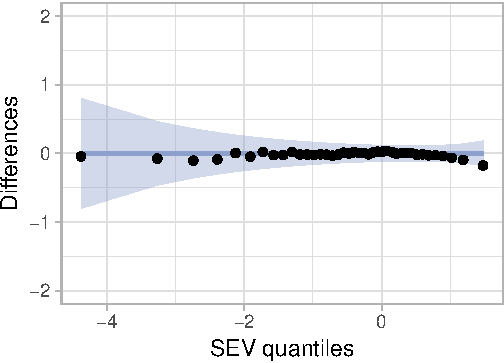
\includegraphics[width=0.45\textwidth]{qqplotr_files/figure-latex/detrend-sev-1} 

}

\caption[An adjusted detrended Q-Q plot assessing the appropriateness of the SEV distribution for the long jump data]{An adjusted detrended Q-Q plot assessing the appropriateness of the SEV distribution for the long jump data.}\label{fig:detrend-sev}
\end{figure}
\end{Schunk}

\begin{Schunk}
\begin{Sinput}
ggplot(longjump, aes(sample = distance)) +
  stat_qq_band(
    distribution = "sev", 
    detrend = TRUE, 
    identity = FALSE,
    dparams = c(mu = 0, sigma = 1),  
    alpha = 0.3
  ) +
  stat_qq_line(
    distribution = "sev", 
    detrend = TRUE, 
    identity = FALSE,
    dparams = c(mu = 0, sigma = 1)
  ) +
  stat_qq_point(
    distribution = "sev", 
    detrend = TRUE,
    identity = FALSE,
    dparams = c(mu = 0, sigma = 1)
  ) +
  xlab("SEV quantiles") +
  ylab("Differences") +
  theme_bw() +
  coord_fixed(ratio = 1)
\end{Sinput}
\end{Schunk}

\subsubsection{BRFSS example}\label{brfss-example}

\label{sec:brfss}

The Center for Disease Control and Prevention runs an annual telephone
survey, the Behavioral Risk Factor Surveillance System (BRFSS), to keep
track of the US populations' ``health-related risk behaviors, chronic
health conditions, and use of preventive services'' \citep{brfss}. Close
to half a million interviews are conducted each year. In this example,
we focus on the responses for Iowa in 2012. The data set consists of
7166 responses across 359 questions and derived variables. To further
illustrate the functionality of \pkg{qqplotr}, we focus on assessing the
distributions of Iowan's heights and weights.

Figure\textasciitilde{}\ref{fig:heights} shows two Q-Q plots side by
side. For each of the plots, a sample of 200 men and 200 women is drawn
from the overall number of responses. On the left hand side,
individuals' heights are plotted in a Q-Q plot comparing raw heights to
a normal distribution. We see that the distributions for both men and
women (colour) show horizontal steps: this indicates that the
distributional assessement is heavily dominated by the discreteness in
the data, as most respondents provided their height to the closest inch.
On the right hand side of Figure\textasciitilde{}\ref{fig:heights}, we
use jittering to remedy this situation---that is, we add a random number
generated from a random uniform distribution on \(\pm 0.5\) inch to the
reported height, as shown in the code below:

\begin{Schunk}
\begin{Sinput}
iowa <- readRDS("data/brfss-iowa.rda")
set.seed(3145)

sample_ia <- iowa %>% 
  tidyr::nest(-SEX) %>% 
  mutate(
    data = data %>% 
    purrr::map(.f = function(x) sample_n(x, size = 200))
    ) %>% 
  tidyr::unnest(data) %>% 
  dplyr::select(SEX, WTKG3, HTIN4) %>%
  mutate(Gender = c("Male", "Female")[SEX])

params <- iowa %>% 
  filter(!is.na(HTIN4)) %>% 
  summarize(
    m = mean(HTIN4),
    s = sd(HTIN4)
  )

customization <- list(scale_fill_brewer(palette="Set1"),
  scale_colour_brewer(palette = "Set1"),
  xlab("Theoretical quantiles"),
  ylab("Height (in inch)"),
  coord_equal(),
  theme_bw(),
  theme(legend.position = c(0.8, 0.2), aspect.ratio = 1))

p1 <- sample_ia %>% 
  ggplot(aes(sample = HTIN4, colour=Gender, fill=Gender)) + 
  stat_qq_band(
    alpha = 0.3, 
    identity = FALSE,
    dparams = list(mean = params$m, sd = params$s)
  ) + 
  stat_qq_line( 
    identity = FALSE,
    dparams = list(mean = params$m, sd = params$s)
  ) + 
  stat_qq_point( 
    dparams = list(mean = params$m, sd = params$s)
  ) +
  customization

p2 <- sample_ia %>% 
  mutate(HTIN4.jitter = jitter(HTIN4, factor = 2)) %>% 
  ggplot(aes(sample = HTIN4.jitter, colour = Gender, fill = Gender)) + 
  geom_abline(slope = 1, intercept = 0, colour = "grey40") +
  stat_qq_band(
    alpha = 0.3, 
    identity = FALSE,
    dparams = list(mean = params$m, sd = params$s)
  ) +
  stat_qq_line(
    identity = FALSE,
    dparams = list(mean = params$m, sd = params$s)
  ) + 
  stat_qq_point(
    dparams = list(mean = params$m, sd = params$s)
  ) +
  customization +
  ylab("Jittered Height (in inch)") 
\end{Sinput}
\end{Schunk}

By using jittering we diminish the effect that discreteness has on the
distribution and brings the observed distribution much closer to a
normal distribution. Note that separate normal distributions were fit to
each gender.
\al{XX I think that we need a note here explaining why we needed to specify dparams rather than letting qqplotr fit the MLEs.}
Unsurprisingly, the resulting distributions have different means (women
are, on average, 6 inches shorter than men in this dataset).
Interestingly, the slope of the two genders is similar, indicating that
the same scale parameter fits both genders' distributions (the standard
deviation of height in the data set is 2.97 inch for men and 2.91 inch
for women, see Table \ref{tab:heights}). The dark line between the two
groups is the identity line, representing the theoretical distribution
each group is compared to. This distribution is based on parameters
estimated from the whole population (see Table \ref{tab:heights} for the
estimates). While the mean is about half way between the gender means,
the standard deviation of the height based on the whole population is
larger, as seen by the steeper slope of the identity compared to the
lines for each group.

\begin{table}

\caption{\label{tab:heights-table}Summary of Iowa residents' heights and weights with corresponding standard deviations by gender and for the total population.\label{tab:heights}}
\centering
\begin{tabular}[t]{lrrrr}
\toprule
SEX & mean height (in inch) & sd (in inch) & mean log weight (in kg) & sd (in kg)\\
\midrule
Male & 70.55 & 2.97 & 9.10 & 0.20\\
Female & 64.51 & 2.91 & 8.89 & 0.23\\
Total & 66.99 & 4.18 & 8.98 & 0.24\\
\bottomrule
\end{tabular}
\end{table}

\begin{Schunk}
\begin{figure}

{\centering 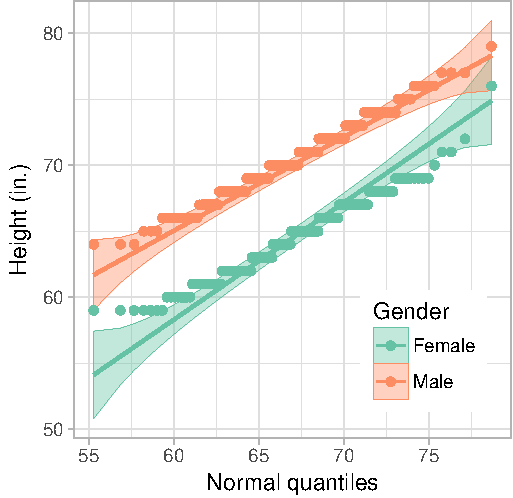
\includegraphics[width=\textwidth]{qqplotr_files/figure-latex/heights-1} 

}

\caption[Q-Q plots comparing the raw (left) and jittered (right) heights to the normal distribution for a sample 200 men and 200 women]{Q-Q plots comparing the raw (left) and jittered (right) heights to the normal distribution for a sample 200 men and 200 women. The distribution on the left is dominated by the discreteness of the data. On the right, using the normal distribution to model people's height is not completely absurd, except for a few extreme outliers.}\label{fig:heights}
\end{figure}
\end{Schunk}

Unlike respondents' heights, their weights do not seem to be normally
distributed. Figure\textasciitilde{}\ref{fig:weights} shows two Q-Q
plots of these data. The Q-Q plot on the left compares raw weights to a
normal distribution. We see that tails of the observed distribution are
heavier than expected under a normal distribution. On the right, weights
are log-transformed. We see that a normal distribution for each of the
genders appears to be reasonable, with the exception of a few extreme
outliers.

\begin{Schunk}
\begin{figure}

{\centering 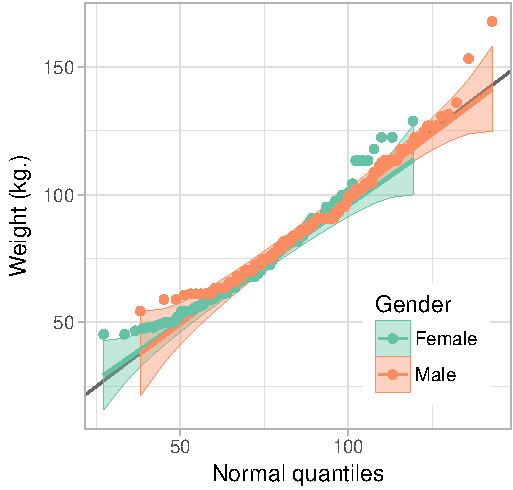
\includegraphics[width=\textwidth]{qqplotr_files/figure-latex/weights-1} 

}

\caption[Q-Q plots comparing weights to the normal distribution for a sample of 200 men and 200 women]{Q-Q plots comparing weights to the normal distribution for a sample of 200 men and 200 women. Unlike people's height, weight seems to be heavily right skewed with some additional outliers in the left tail (left plot). On the right, weight was log-transfomed before its distribution is compared to a theoretical normal.}\label{fig:weights}
\end{figure}
\end{Schunk}

Instead of log-transforming the observed weights, we can change the
theoretical distribution to a lognormal.
Figure\textasciitilde{}\ref{fig:weights-log} shows two lognormal Q-Q
plots, one for each gender. note that by default, the MLEs are used to
parameterize the lognormal distribution for each group:

\begin{Schunk}
\begin{Sinput}
p4 <- sample_ia %>% 
  ggplot(aes(sample = WTKG3 / 100, colour = Gender, fill = Gender)) +
  geom_abline(colour = "grey40") +
  stat_qq_band(
    distribution = "lnorm",
    dparams = list(meanlog = mlog, sdlog = sdlog),
    alpha = 0.3
  ) +
  stat_qq_line(
    distribution = "lnorm",
    dparams = list(meanlog = mlog, sdlog = sdlog)
  ) +
  stat_qq_point(
    distribution = "lnorm",
    dparams = list(meanlog = mlog, sdlog = sdlog)
  ) +
  customization +
  theme(legend.position = c(0.2, 0.8)) 

p6 <- sample_ia %>% 
  ggplot(aes(sample = WTKG3 / 100, colour = Gender, fill = Gender)) +
  geom_abline(colour = "grey40") +
  stat_qq_band(
    distribution = "lnorm", 
    alpha = 0.3
  ) +
  stat_qq_line(
    distribution = "lnorm"
  ) +
  stat_qq_point(
    distribution = "lnorm"
  ) +
  customization + facet_grid(. ~ Gender)
\end{Sinput}
\begin{figure}

{\centering 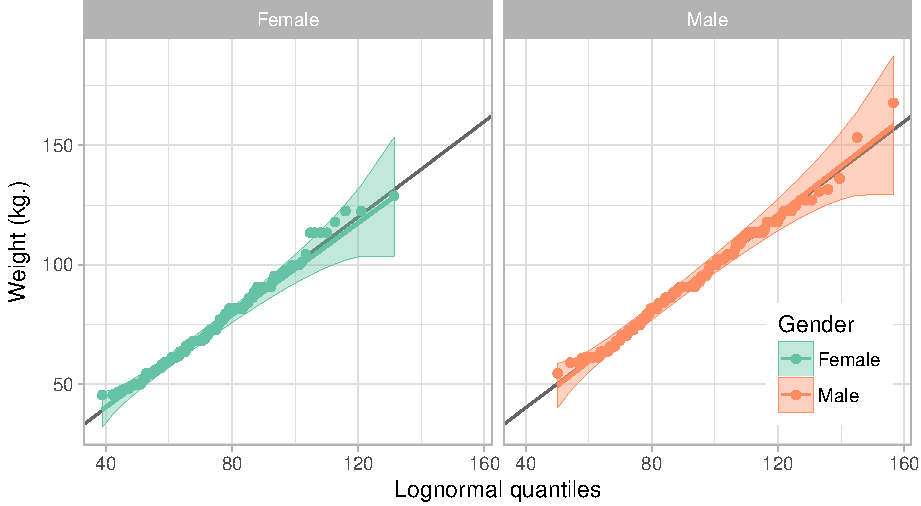
\includegraphics[width=.9\textwidth]{qqplotr_files/figure-latex/weights-log-1} 

}

\caption[Q-Q plots comparing weights to a lognormal distribution for a sample of 200 men and 200 women]{Q-Q plots comparing weights to a lognormal distribution for a sample of 200 men and 200 women. Shift and scale parameters are estimated separately for each of the genders before comparing distributions to a log-normal.}\label{fig:weights-log}
\end{figure}
\end{Schunk}

\subsection{Discussion}\label{discussion}

This paper presents the \pkg{qqplotr} package, an extension of
\pkg{ggplot2} that implements Q-Q plots in both the standard and
detrended orientations, along with reference lines and confidence bands.
The examples illustrate how to create Q-Q plots for non-standard
distributions found outside of the \pkg{stats} package, how to create
detrended Q-Q plots, and how to create Q-Q plots when data are grouped.
Further, in the BRFSS example, we illustrated how jittering can be used
in Q-Q plots to better compare discretized data to a continuous
distribution.

Q-Q plots are members of the larger probability plotting family, and
future versions of \pkg{qqplotr} will incorporate additional plots.
Specifically, two types of probability plots will be included:

\begin{enumerate}
\def\labelenumi{\arabic{enumi}.}
\tightlist
\item
  A standardarized P-P plot is constructed for location-scale
  distributions by plotting \(F(z_{(i)})\) against \(p_i\), where
  \(z_{(i)}\) denotes the ordered and standardized observations and
  \(p_i\) denotes the plotting position \citep{Gan1991-yk}. As
  \citet{Gan1991-yk} point out, the probability plotting positions are
  equally spaced on the \(x\)-axis, whereas points on the \(x\)-axis of
  a Q-Q plot are more concentrated in the higher-density regions of the
  reference distribution. This leads to Q-Q plots being more sensitive
  to discrepancies in the tails of the distribution and standardized P-P
  plots being more sensitive to discrepancies in the ``middle'' of the
  proposed distribution.
\item
  In engineering applications, probability plots refer to a linearized
  plot of \(F(x_i)\) against \(x_i\). The linearizing transformation of
  the hypothesized CDF is found by first finding a transformation that
  linearizes the quantile function---i.e., linearizing the plot of
  \(F^{-1}(p)\) vs. \(x_p\)---and then mapping \(F^{-1}(p)\) back to the
  probability scale \citep[cf.][Chapter 6]{Meeker1998}.
\end{enumerate}

It is important to note that all of the probability plotting methods
discussed---Q-Q plots, standardized P-P plots, and probability
plots---are invariant to linear transformations. Consequently, each type
of plot will exhibit a linear relationship between the sample and
hypothesized distribution for location-scale families, even if the
location and/or scale parameters in the sample differ from the
hypothesized distribution. This is not the case with unstandardized P-P
plots \citep{Wilk1968-ii}, so they will not be included in
\pkg{qqplotr}.

Finally, we have made design choices in \pkg{qqplotr} that we believe
are in line with best practices for distributional assessment, but the
implementation is flexible enough to allow for easy customization. For
example, maximum likelihood estimation is used to estimate the
parameters of the proposed model, but if outliers are present robust
estimators may be desirable, such as if you are comparing the empirical
distribution to a normal distribution. In this scenario, robust
estimates of the location and scale can be obtained using the
\pkg{robustbase} package \citep{robustbase}, and specified using the
\texttt{dparams} parameter directly. This is especially useful if you
wish to use the parametric bootstrap to build confidence bands.
Similarly, \texttt{stat\_qq\_line} implements two types of reference
lines: the identity line, and another that passes through two quantiles
of the distributions, such as the first and third quartiles. While those
are the most traditional used reference lines, alternative ones can be
quickly implemented using \texttt{ggplot2::geom\_abline} by specifying
the slope and intercept.

\bibliography{RJreferences}

\subsection{Acknowledgements}\label{acknowledgements}

This work was partially funded by Google Summer of Code 2017.

\address{%
Alexandre Almeida\\
University of Campinas\\
Institute of Computing\\ Campinas, Brazil 13083-852\\
}
\href{mailto:almeida.xan@gmail.com}{\nolinkurl{almeida.xan@gmail.com}}

\address{%
Adam Loy\\
Carleton College\\
Department of Mathematics and Statistics\\ Northfield, MN 55057\\
}
\href{mailto:aloy@carleton.edu}{\nolinkurl{aloy@carleton.edu}}

\address{%
Heike Hofmann\\
Iowa State University\\
Department of Statistics\\ Ames, IA 50011-1210\\
}
\href{mailto:hofmann@iastate.edu}{\nolinkurl{hofmann@iastate.edu}}

